%% AMS-LaTeX Created with the Wolfram Language : www.wolfram.com

\documentclass{article}
\usepackage{amsmath, amssymb, graphics, setspace}

\newcommand{\mathsym}[1]{{}}
\newcommand{\unicode}[1]{{}}

\newcounter{mathematicapage}
\begin{document}

\title{Curva de Rota{\c c}{\~ a}o ESO 116-G12}
\author{}
\date{}
\maketitle

\section*{Utilit{\' a}rios}

\begin{doublespace}
\noindent\(\pmb{\text{}}\)
\end{doublespace}

Massa Solar $\to $ Grama \\
\(\(\)\)\\
\(\(\text{Kpc} \to  \text{Cm} \\
\\\)\)\\
\(\(\text{Densidades}\\
\\\)\)

\section*{Tabelas}

\begin{doublespace}
\noindent\(\pmb{\text{data}= }\\
\pmb{\text{Import}[}\\
\pmb{\text{{``}C:$\backslash \backslash $Users$\backslash \backslash $Leoleo$\backslash \backslash $Desktop$\backslash \backslash $TCC$\backslash \backslash $Mathematica$\backslash \backslash $Fitting$\backslash \backslash $116.dat{''}}];}\\
\pmb{\text{RC}_{\text{total}}=\text{Table}[\{\text{data}[[i,1]],\text{data}[[i,3]]\},\{i,1,15\}];}\\
\pmb{\text{RC}_{\text{gas}}=\text{Table}[\{\text{data}[[i,1]],\text{data}[[i,4]]\},\{i,1,15\}];}\\
\pmb{\text{Erro} = \text{Table}[\text{data}[[i,5]],\{i,1,15\}];}\\
\pmb{\text{radii}=\text{Part}[\text{Transpose}[\text{data}],1];}\\
\pmb{\text{Vel}=\text{Part}[\text{Transpose}[\text{data}],3];}\\
\pmb{\text{err}=\text{Part}[\text{Transpose}[\text{data}],5];}\\
\pmb{}\\
\pmb{\text{TableForm}[\text{data},}\\
\pmb{\text{TableHeadings}\to \{\{\text{{``}{''}}\},\{\text{{``}Raio{''}},\text{{``}{''}},\text{{``}Vtotal{''}},\text{{``}Vgas{''}},\text{{``}Erro{''}}\}\}]}\)
\end{doublespace}

\begin{doublespace}
\noindent\(\begin{array}{l|l|llll}
  & \text{Raio} & \text{} & \text{Vtotal} & \text{Vgas} & \text{Erro} \\
\hline
 \text{} & 0.295522 & 7.58904 & 20.94 & -0.234178 & 3.4 \\
\hline
  & 0.985821 & 7.79329 & 39.95 & -1.95065 & 3.29 \\
  & 1.62537 & 8.47973 & 51.54 & -1.68024 & 2.96 \\
  & 2.18881 & 9.15955 & 67.92 & 5.43454 & 3.45 \\
  & 3.17687 & 9.76846 & 80.22 & 13.5993 & 2.93 \\
  & 3.76791 & 9.48569 & 83.33 & 18.0705 & 3.08 \\
  & 4.35896 & 8.74732 & 91.38 & 21.8567 & 2.83 \\
  & 4.8903 & 7.95629 & 101.65 & 24.2219 & 5.4 \\
  & 6.19403 & 6.20847 & 104.77 & 27.7912 & 4.21 \\
  & 7.16418 & 5.25717 & 108.62 & 29.5757 & 2.1 \\
  & 8.0597 & 4.68539 & 108.48 & 30.9882 & 2.1 \\
  & 8.95522 & 4.27244 & 108.73 & 33.3072 & 2.1 \\
  & 9.85075 & 3.43065 & 110.24 & 36.6602 & 2.1 \\
  & 10.7463 & 1.87414 & 110.63 & 38.4926 & 2.33 \\
  & 11.6418 & 0.66706 & 111.52 & 36.585 & 4.74 \\
\end{array}\)
\end{doublespace}

\subsection*{}

\section*{Valores de Par{\^ a}metros}

\begin{doublespace}
\noindent\(\pmb{\text{Tabela}_{\text{Vdisk}}=}\\
\pmb{\text{TableForm}[}\\
\pmb{P_{\text{stars}}= \left\{\left\{10^{0.2},10^9\right\},\left\{10^{0.3},10^{9.8}\right\},\left\{10^{0.4},10^{10.4}\right\},\left\{10^{0.7},10^{11}\right\}\right\},}\\
\pmb{\left.\text{TableHeadings}\to \left\{\{\text{{``}1{''}},\text{{``}2{''}},\text{{``}3{''}},\text{{``}4{''}}\},\left\{\texttt{"}R_d\texttt{"},\texttt{"}M_d\texttt{"}\right\}\right\}\right];}\\
\pmb{\text{Tabela}_{\text{Vdm} }=}\\
\pmb{\text{TableForm}[}\\
\pmb{P_{\text{dm}}=\left\{\left\{10^{-0.5},4.1*10^8\right\},\left\{1,1.05*10^8\right\},\left\{10^{0.5},2.5*10^7\right\},\right.}\\
\pmb{\left\{10^{0.8},9.7*10^6\right\},\left\{10,5.7*10^6\right\},\left\{10^{1.2},3.9*10^6\right\},}\\
\pmb{\left.\left\{10^{1.4},2.3*10^6\right\},\left\{10^{1.6},1.4*10^6\right\}\right\},}\\
\pmb{\text{TableHeadings}\to \{\{\text{{``}Dwarf Spiral{''}},\text{{``}{''}},\text{{``}{''}},\text{{``}Spiral Galaxy{''}}\},}\\
\pmb{\left.\left.\left\{\texttt{"}R_0\texttt{"},\texttt{"}P_0\texttt{"}\right\}\right\}\right];}\\
\pmb{G\text{:=}\frac{4.302}{10^6};}\\
\pmb{}\\
\pmb{\left\{\text{Tabela}_{\text{Vdisk}},\text{Tabela}_{\text{Vdm}}\right\}}\)
\end{doublespace}

\begin{doublespace}
\noindent\(\left\{
\begin{array}{l|l|l}
  & R_d & M_d \\
\hline
 1 & 1.58489 & 1000000000 \\
\hline
 2 & 1.99526 & 6.30957\times 10^9 \\
 3 & 2.51189 & 2.51189\times 10^{10} \\
 4 & 5.01187 & 100000000000 \\
\end{array}
,
\begin{array}{l|l|l}
  & R_0 & P_0 \\
\hline
 \text{Dwarf Spiral} & 0.316228 & 4.1\times 10^8 \\
\hline
 \text{} & 1 & 1.05\times 10^8 \\
 \text{} & 3.16228 & 2.5\times 10^7 \\
 \text{Spiral Galaxy} & 6.30957 & 9.7\times 10^6 \\
  & 10 & 5.7\times 10^6 \\
  & 15.8489 & 3.9\times 10^6 \\
  & 25.1189 & 2.3\times 10^6 \\
  & 39.8107 & 1.4\times 10^6 \\
\end{array}
\right\}\)
\end{doublespace}

\section*{Conversor de Unidades}

\begin{doublespace}
\noindent\(\pmb{\text{ConversorKpc} =\text{DynamicModule}[\{a=0,b=0\},}\\
\pmb{\text{Deploy}[}\\
\pmb{\text{Style}[}\\
\pmb{\text{Panel}[}\\
\pmb{\text{Grid}[\text{Transpose}[}\\
\pmb{\{\{\text{Style}[\text{{``}Valor em Cm{''}},\text{Red}],\text{Style}[\text{{``}Valor em Kpc{''}},\text{Blue}],}\\
\pmb{\text{{``}Valor em Kpc{''}}, \text{{``}Valor em Cm{''}}\},}\\
\pmb{\{\text{InputField}[\text{Dynamic}[a],\text{Number}],}\\
\pmb{\text{InputField}[\text{Dynamic}[b],\text{Number}],}\\
\pmb{\text{InputField}\left[\text{Dynamic}\left[N\left[a\left/\left(3.08*10^{21}\right)\right.\right]\right]\right],}\\
\pmb{\left.\left.\left.\left.\text{InputField}\left[\text{Dynamic}\left[b*\left(3.08*10^{21}\right)\right],\text{Enabled}\to \text{False}\right]\right\}\right\}\right]\right],}\\
\pmb{\text{Alignment}\to \text{Right},\text{ImageMargins}\to 10],}\\
\pmb{\text{DefaultOptions}\to }\\
\pmb{\{\text{InputField}\to \{\text{FieldSize}\{\{5,30\},\{1,\text{Infinity}\}\}\}\}]]];}\\
\pmb{}\\
\pmb{\text{ConversorMsol} =\text{DynamicModule}[\{a=0,b=0\},}\\
\pmb{\text{Deploy}[}\\
\pmb{\text{Style}[}\\
\pmb{\text{Panel}[}\\
\pmb{\text{Grid}[\text{Transpose}[}\\
\pmb{\{\{\text{Style}[\text{{``}Massa Solar{''}},\text{Red}],\text{Style}[\text{{``}Grama{''}},\text{Blue}],}\\
\pmb{\text{{``}Valor em Grama{''}}, \text{{``}Valor em Msol{''}}\},}\\
\pmb{\{\text{InputField}[\text{Dynamic}[a],\text{Number}],}\\
\pmb{\text{InputField}[\text{Dynamic}[b],\text{Number}],}\\
\pmb{\text{InputField}\left[\text{Dynamic}\left[N\left[a*\left(1.99*10^{33}\right)\right]\right]\right],}\\
\pmb{\left.\left.\left.\left.\text{InputField}\left[\text{Dynamic}\left[N\left[b\left/\left(1.99*10^{33}\right)\right.\right]\right],\text{Enabled}\to \text{False}\right]\right\}\right\}\right]\right],}\\
\pmb{\text{Alignment}\to \text{Right},\text{ImageMargins}\to 10],}\\
\pmb{\text{DefaultOptions}\to }\\
\pmb{\{\text{InputField}\to \{\text{FieldSize}\{\{5,30\},\{1,\text{Infinity}\}\}\}\}]]];}\\
\pmb{\text{ConversorDensidade} =\text{DynamicModule}[\{a=0,b=0\},}\\
\pmb{\text{Deploy}[}\\
\pmb{\text{Style}[}\\
\pmb{\text{Panel}[}\\
\pmb{\text{Grid}\left[\text{Transpose}\left[\left\{\left\{\text{Style}\left[\text{$\texttt{"}$Densidade em }\frac{\text{Msol}}{\text{Kpc}^3}\texttt{"},\text{Red}\right],\right.\right.\right.\right.}\\
\pmb{\left.\text{Style}\left[\text{$\texttt{"}$Densidade em }\frac{g}{\text{cm}^3}\texttt{"},\text{Blue}\right],\texttt{"}\frac{g}{\text{Cm}^3}\texttt{"}, \texttt{"}\frac{\text{Msol}}{\text{Kpc}^3}\texttt{"}\right\},}\\
\pmb{\{\text{InputField}[\text{Dynamic}[a]],\text{InputField}[\text{Dynamic}[b]],}\\
\pmb{\text{InputField}\left[\text{Dynamic}\left[N\left[a*\left(6.47*10^{-32}\right)\right]\right]\right],}\\
\pmb{\left.\left.\left.\left.\text{InputField}\left[\text{Dynamic}\left[N\left[b*\left(1.5*10^{31}\right)\right]\right],\text{Enabled}\to \text{False}\right]\right\}\right\}\right]\right],}\\
\pmb{\text{Alignment}\to \text{Right},\text{ImageMargins}\to 10],}\\
\pmb{\text{DefaultOptions}\to }\\
\pmb{\{\text{InputField}\to \{\text{FieldSize}\{\{5,30\},\{1,\text{Infinity}\}\}\}\}]]];}\)
\end{doublespace}

\section*{Equa{\c c}{\~ o}es}

\subsubsection*{Velocidade das Estrelas no Disco}

\begin{doublespace}
\noindent\(\pmb{V^2{}_{\text{disk}}[\text{r$\_$}]=}\\
\pmb{\frac{1}{2 R_d}}\\
\pmb{\left(G M_d \left(\frac{r}{R_d}\right){}^2\right) }\\
\pmb{\left(\text{BesselI}\left[0,\frac{r}{2 R_d}\right] \text{BesselK}\left[0,\frac{r}{2 R_d}\right]-\right.}\\
\pmb{\left.\text{BesselI}\left[1,\frac{r}{2 R_d}\right] \text{BesselK}\left[1,\frac{r}{2 R_d}\right]\right);}\)
\end{doublespace}

\subsubsection*{Velocidade Mat{\' e}ria Escura}

\begin{doublespace}
\noindent\(\pmb{V^2{}_{\text{Dm}}[\text{r$\_$}]=\frac{6.4 G \left(P_o R_o^3\right) \left(\frac{1}{2} \text{Log}\left[\left(\frac{r}{R_o}\right){}^2+1\right]+\text{Log}\left[\frac{r}{R_o}+1\right]-\text{ArcTan}\left[\frac{r}{R_o}\right]\right)}{r};}\)
\end{doublespace}

\subsubsection*{\\
Velocidade Total}

\begin{doublespace}
\noindent\(\pmb{V_t[\text{r$\_$}]=\text{Sqrt}\left[V^2{}_{\text{disk}}[r]+V^2{}_{\text{Dm}}[r]+\text{Igas}[r]^2\right];}\)
\end{doublespace}

\section*{Interpola{\c c}{\~ a}o do G{\' a}s}

\begin{doublespace}
\noindent\(\pmb{\text{Igas}=\text{Interpolation}\left[\text{RC}_{\text{gas}}\right];}\\
\pmb{V^2{}_{\text{gas}}=\text{Igas}^2[r];}\\
\pmb{\text{Gas}= \text{Plot}[\text{Igas}[x],\{x,1.8,11.7\},\text{AxesOrigin}\to \{x=0,x=0\},}\\
\pmb{\text{PlotStyle}\to \{\text{Black},\text{Dashed}\},\text{AxesLabel}\to \{\text{{``}R(Kpc){''}},\text{{``}V(Kpc){''}}\}]}\)
\end{doublespace}

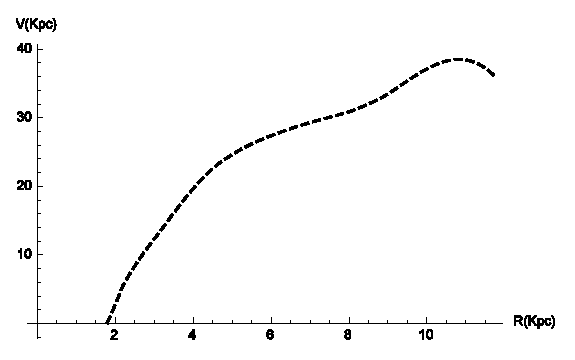
\includegraphics{Ajuste_gr1.eps}

\section*{Gr{\' a}fico Velocidade das estrelas no disco}

\begin{doublespace}
\noindent\(\pmb{V_{\text{d1}}=\text{Plot}\left[\sqrt{V^2{}_{\text{disk}}[r]}\text{/.}\, \left\{R_d\to 1.58,M_d\to 10^9\right\},\{r,0,20\}\right] ;}\\
\pmb{V_{\text{d2}}=\text{Plot}\left[\sqrt{V^2{}_{\text{disk}}[r]}\text{/.}\, \left\{R_d\to 1.99,M_d\to 6.3*10^9\right\},\{r,0,30\}\right] ;}\\
\pmb{V_{\text{d3}}=\text{Plot}\left[\sqrt{V^2{}_{\text{disk}}[r]}\text{/.}\, \left\{R_d\to 2.51,M_d\to 2.5*10^{10}\right\},\{r,0,40\}\right] ;}\\
\pmb{V_{\text{d4}}=\text{Plot}\left[\sqrt{V^2{}_{\text{disk}}[r]}\text{/.}\, \left\{R_d\to 5.01,M_d\to 10^{11}\right\},\{r,0,50\}\right] ;}\\
\pmb{V_{d }=\text{Show}\left[V_{\text{d1}},V_{\text{d2}},V_{\text{d3}},V_{\text{d4}},\text{Frame}\text{-$>$}\text{True},\text{PlotRange}\text{-$>$}\text{All},\right.}\\
\pmb{\text{AspectRatio}\to 0.8,\text{PlotLabel}\to \text{{``}Estrelas no disco{''}},}\\
\pmb{\text{AxesLabel}\to \{\text{{``}R(Kpc){''}},\text{{``}V(Km/s){''}}\}];}\)
\end{doublespace}

\section*{Gr{\' a}fico Velocidade Mat{\' e}ria Escura}

\begin{doublespace}
\noindent\(\pmb{V_{\text{dm1}}=\text{Plot}\left[\sqrt{V^2{}_{\text{Dm}}[r]}\text{/.}\, \left\{R_o\to 0.32,P_o\to 4.1\ 10^8\right\},\{r,0,10\},\right.}\\
\pmb{\text{PlotRange}\to \text{All}];}\\
\pmb{V_{\text{dm2}}=\text{Plot}\left[\sqrt{V^2{}_{\text{Dm}}[r]}\text{/.}\, \left\{R_o\to 1,P_o\to 1.05\ 10^8\right\},\{r,0,12\},\right.}\\
\pmb{\text{PlotRange}\text{-$>$}\text{All}];}\\
\pmb{V_{\text{dm3}}=\text{Plot}\left[\sqrt{V^2{}_{\text{Dm}}[r]}\text{/.}\, \left\{R_o\to 3.16,P_o\to 2.5\ 10^7\right\},\{r,0,20\},\right.}\\
\pmb{\text{PlotRange}\to \text{All}];}\\
\pmb{V_{\text{dm4}}=\text{Plot}\left[\sqrt{V^2{}_{\text{Dm}}[r]}\text{/.}\, \left\{R_o\to 6.31,P_o\to 9.7\ 10^6\right\},\{r,0,45\},\right.}\\
\pmb{\text{PlotRange}\to \text{All}];}\\
\pmb{V_{\text{dm5}}=\text{Plot}\left[\sqrt{V^2{}_{\text{Dm}}[r]}\text{/.}\, \left\{R_o\to 10,P_o\to 5.7\ 10^6\right\},\{r,0,60\},\right.}\\
\pmb{\text{PlotRange}\to \text{All}];}\\
\pmb{V_{\text{dm6}}=\text{Plot}\left[\sqrt{V^2{}_{\text{Dm}}[r]}\text{/.}\, \left\{R_o\to 15.85,P_o\to 3.9\ 10^6\right\},\{r,0,70\},\right.}\\
\pmb{\text{PlotRange}\to \text{All}];}\\
\pmb{V_{\text{dm7}}= \text{Plot}\left[\sqrt{V^2{}_{\text{Dm}}[r]}\text{/.}\, \left\{R_o\to 25.12,P_o\to 2.3\ 10^6\right\},\{r,0,100\},\right.}\\
\pmb{\text{PlotRange}\to \text{All}];}\\
\pmb{V_{\text{dm8}}=\text{Plot}\left[\sqrt{V^2{}_{\text{Dm}}[r]}\text{/.}\, \left\{R_o\to 39.81,P_o\to 1.4\ 10^6\right\},\{r,0,125\},\right.}\\
\pmb{\text{PlotRange}\to \text{All}];}\\
\pmb{\text{Show}\left[V_{\text{dm1}},V_{\text{dm2}},V_{\text{dm3}}\right];}\\
\pmb{V_{\text{dm} }=\text{Show}\left[V_{\text{dm4}},V_{\text{dm5}},V_{\text{dm6}},V_{\text{dm7}},V_{\text{dm8}}, \text{Frame}\to \text{True},\text{PlotRange}\text{-$>$}\text{All},\right.}\\
\pmb{\text{AspectRatio}\to 0.75,}\\
\pmb{\text{PlotLabel}\to \text{{``}Modelo de Burket para o Halo de Mat{\' e}ria Escura{''}}];}\\
\pmb{}\)
\end{doublespace}

\section*{Modelo de Burket ESO 116-G12}

\begin{doublespace}
\noindent\(\pmb{\text{Needs}[\text{{``}ErrorBarPlots$\grave{ }${''}}];}\\
\pmb{\text{CR}_{\text{tot}}=\text{ErrorListPlot}\left[\left\{\text{Table}\left[\left\{\text{RC}_{\text{total}}[[i]],\text{ErrorBar}[\text{Erro}[[i]]]\right\},\{i,15\}\right]\right\},\right.}\\
\pmb{\text{PlotStyle}\to \text{Black},\text{MeshStyle}\to \text{PointSize}[\text{Large}]];}\\
\pmb{\text{RC}_{\text{stars}}=\text{Plot}\left[\sqrt{V^2{}_{\text{disk}}[r]}\text{/.}\, \left\{M_d\to 2.4\ 10^9,R_d\to 1.7\right\},\{r,0,11.7\},\right.}\\
\pmb{\text{PlotStyle}\to \{\text{Black},\text{Dotted}\}];}\\
\pmb{\text{RC}_{\text{halo}}=\text{Plot}\left[\sqrt{V^2{}_{\text{Dm}}[r]}\text{/.}\, \left\{R_o\to 4.3,P_o\to 4.7\ 10^7\right\},\{r,0,11.7\},\right.}\\
\pmb{\text{PlotStyle}\to \{\text{Black},\text{DotDashed}\}];}\\
\pmb{\text{RC}_{\text{vtot}}=\text{Plot}\left[V_t[r]\text{/.}\left\{M_d\to 2.4\ 10^9,R_d\to 1.7,R_o\to 4.3,P_o\to 4.7\ 10^7\right\},\right.}\\
\pmb{\{r,0.3,11.6\},\text{PlotStyle}\to \text{Black},\text{PlotRange}\to \text{Automatic}];}\\
\pmb{\text{Show}\left[\text{CR}_{\text{tot}},\text{RC}_{\text{stars}},\text{RC}_{\text{halo}},\text{RC}_{\text{vtot}},\text{Gas},\text{Frame}\to \text{True},\right.}\\
\pmb{\text{PlotRange}\to \{\{0,11.6\},\{0,115\}\},\text{PlotLabel}\to \text{{``}ESO 116-G12{''}},}\\
\pmb{\text{FrameLabel}\to \{\text{{``}R(Kpc){''}},\text{{``}V(Km/s){''}}\}]}\\
\pmb{\text{Table}\left[\left\{V_d,V_{\text{dm}}\right\}\right]}\)
\end{doublespace}

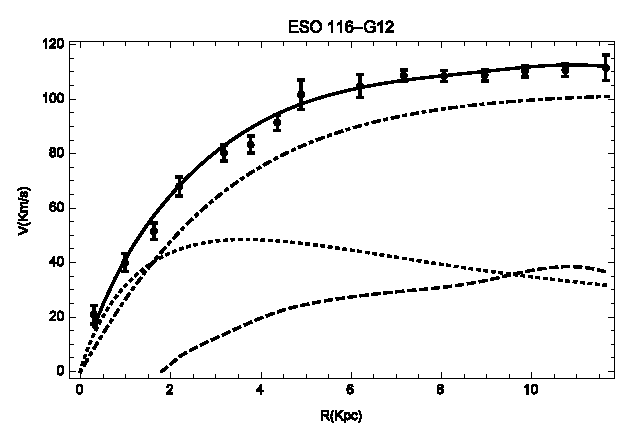
\includegraphics{Ajuste_gr2.eps}

\begin{doublespace}
\noindent\(\{,\}\)
\end{doublespace}

\section*{Ajuste Linear}

\begin{doublespace}
\noindent\(\pmb{\text{}}\\
\pmb{\text{Clear}[x]}\)
\end{doublespace}

\begin{doublespace}
\noindent\(\pmb{f[\text{x$\_$},\text{c$\_$},\text{d$\_$}]\text{:=}c+d*x;}\\
\pmb{\text{data}_a = \text{Table}[\{2,4,5,9,13,14.5,15.8,16.4,18,21.4\}];}\\
\pmb{\text{LMF} =\text{LinearModelFit}\left[\text{data}_a,x,x\right]}\\
\pmb{\text{   }\text{Ajuste} =\text{Show}\left[\text{ListPlot}\left[\text{data}_a,\text{PlotStyle}\to \text{Red}\right],\right.}\\
\pmb{\text{Plot}[\text{LMF}[x],\{x,0,10\}]]}\\
\pmb{\text{Ajuste}_{1 }=\text{NonlinearModelFit}\left[\text{data}_a,f[x,c,d],\{\{c,0.5\},\{d,3\}\},x\right]}\\
\pmb{\text{Clear}[f];}\)
\end{doublespace}

\begin{doublespace}
\noindent\(\text{FittedModel}[]\)
\end{doublespace}

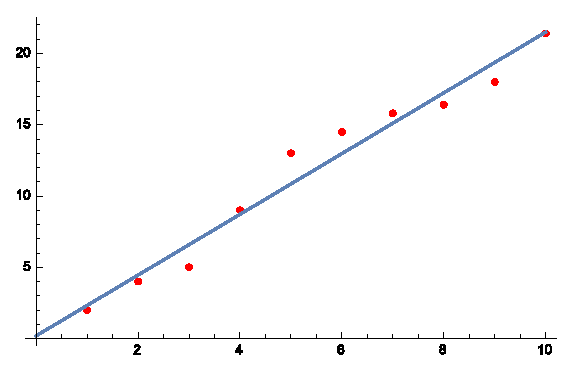
\includegraphics{Ajuste_gr3.eps}

\begin{doublespace}
\noindent\(\text{FittedModel}[]\)
\end{doublespace}

\begin{doublespace}
\noindent\(\pmb{f[\text{x$\_$},\text{a$\_$},\text{b$\_$},\text{c$\_$}]\text{:=}a+b*x+c*x^2;}\\
\pmb{\text{datab} = }\\
\pmb{\text{Table}[\{\{-2,5\},\{-1.8,4.3\},\{-1.5,2.5\},\{-1.2,2\},\{-1,1\},}\\
\pmb{\{-0.7,0.8\},\{-0.5,0.9\},\{-0.3,1.4\},\{0,2\},\{0.2,2.4\},}\\
\pmb{\{0.3,3\},\{0.5,4\},\{0.6,5\}\}];}\\
\pmb{\text{Fit}_1 =\text{NonlinearModelFit}[\text{datab},f[x,b,c,a],\{\{a,2\},\{b,4\},\{c,2\}\},}\\
\pmb{x]}\\
\pmb{\text{Show}\left[\text{ListPlot}[\text{datab},\text{PlotStyle}\to \text{Red}],\text{Plot}\left[\text{Fit}_1[r],\{r,-5,5\}\right]\right]}\\
\pmb{\text{Clear}[f];}\)
\end{doublespace}

\begin{doublespace}
\noindent\(\text{FittedModel}\left[\right]\)
\end{doublespace}

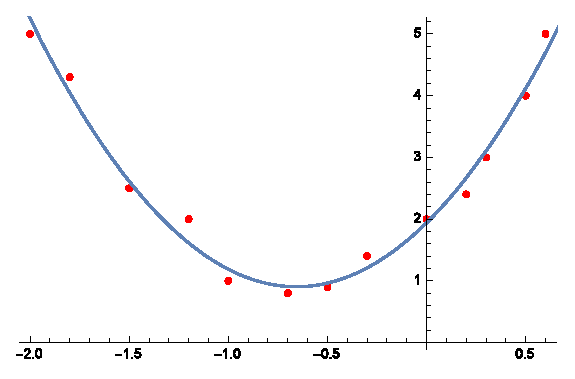
\includegraphics{Ajuste_gr4.eps}

\section*{Ajuste N{\~ a}o Linear}

\begin{doublespace}
\noindent\(\pmb{\text{Clear}[f]}\\
\pmb{\text{VDisk}[\text{r$\_$},\text{M$\_$}]\text{:=}\frac{1}{2 R_d}\left(G (M*10{}^{\wedge}9) \left(\frac{r}{R_d}\right){}^2\right) }\\
\pmb{\left(\text{BesselI}\left[0,\frac{r}{2 R_d}\right] \text{BesselK}\left[0,\frac{r}{2 R_d}\right]-\right.}\\
\pmb{\left.\text{BesselI}\left[1,\frac{r}{2 R_d}\right] \text{BesselK}\left[1,\frac{r}{2 R_d}\right]\right);}\\
\pmb{\text{VDark}[\text{r$\_$},\text{R$\_$},\text{P$\_$}]\text{:=}}\\
\pmb{\frac{6.4 G \left((P *10{}^{\wedge}7) R^3\right) \left(\frac{1}{2} \text{Log}\left[\left(\frac{r}{R}\right)^2+1\right]+\text{Log}\left[\frac{r}{R}+1\right]-\text{ArcTan}\left[\frac{r}{R}\right]\right)}{r};}\\
\pmb{h[\text{r$\_$},\text{R$\_$},\text{P$\_$},\text{M$\_$}]\text{:=} \text{Sqrt}[\text{VDisk}[r,M]+\text{VDark}[r,R,P]];}\\
\pmb{R_d\text{:=}1.7;}\\
\pmb{}\\
\pmb{\text{Fit2}=\text{NonlinearModelFit}\left[\text{RC}_{\text{total}},h[r,R,P,M],\right.}\\
\pmb{\{\{M,0.1,10\},\{P,0.1,10\},\{R,1,10\}\},r]}\\
\pmb{\text{Fit2}[\text{{``}ParameterTable{''}}]}\\
\pmb{\text{Show}\left[\text{ListPlot}\left[\text{RC}_{\text{total}}\right],\text{Plot}[\text{Fit2}[r],\{r,0,100\},\text{AxesOrigin}\to \{0,0\}]\right]}\)
\end{doublespace}

\begin{doublespace}
\noindent\(\text{FittedModel}\left[\right]\)
\end{doublespace}

\begin{doublespace}
\noindent\(\begin{array}{l|llll}
 \text{} & \text{Estimate} & \text{Standard Error} & \text{t-Statistic} & \text{P-Value} \\
\hline
 M & 2.06848 & 0.687315 & 3.00951 & 0.0108728 \\
 P & 4.63667 & 1.15787 & 4.00447 & 0.00174759 \\
 R & 4.66305 & 0.626713 & 7.44048 & \text{7.835084657999502$\grave{ }$*${}^{\wedge}$-6} \\
\end{array}\)
\end{doublespace}

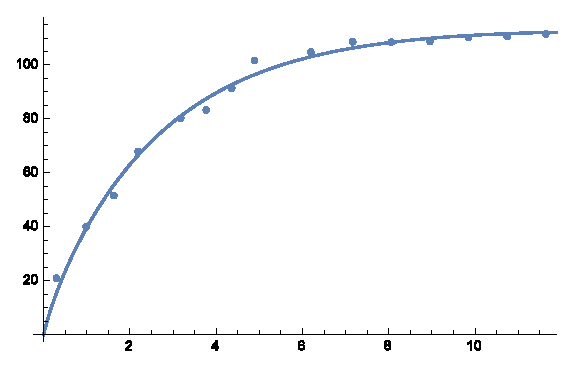
\includegraphics{Ajuste_gr5.eps}

\begin{doublespace}
\noindent\(\pmb{\text{}}\\
\pmb{}\\
\pmb{}\\
\pmb{j[\text{r$\_$},\text{R$\_$},\text{P$\_$},\text{M$\_$}]\text{:=}\text{Sqrt}\left[\text{VDisk}[r,M]+\text{VDark}[r,R,P]+\text{Igas}[r]^2\right]}\\
\pmb{\text{Fit3}=\text{NonlinearModelFit}\left[\text{RC}_{\text{total}},j[r,R,P,M],\right.}\\
\pmb{\{\{M,0.1,10\},\{P,0.1,10\},\{R,1,10\}\},r,\text{Weights}\to 1/\text{err}{}^{\wedge}2]}\\
\pmb{\text{Fit3}[\text{{``}ParameterTable{''}}]}\\
\pmb{\text{Show}\left[\text{ListPlot}\left[\text{RC}_{\text{total}}\right],\text{Plot}[\text{Fit3}[r],\{r,0,100\},\text{AxesOrigin}\to \{0,0\}]\right]}\)
\end{doublespace}

\begin{doublespace}
\noindent\(\text{FittedModel}\left[\right]\)
\end{doublespace}

\begin{doublespace}
\noindent\(\begin{array}{l|llll}
 \text{} & \text{Estimate} & \text{Standard Error} & \text{t-Statistic} & \text{P-Value} \\
\hline
 M & 2.08205 & 0.735815 & 2.82959 & 0.0151873 \\
 P & 4.51678 & 1.32533 & 3.40803 & 0.0051921 \\
 R & 4.40809 & 0.670834 & 6.57106 & 0.0000264688 \\
\end{array}\)
\end{doublespace}

